\chapter{Résumé}

\minitoc[n] % minitoc without title

\section{Introduction}

	\subsection{La Coopération} % TODO: changer

		% TODO : Dire qu'on utilise autant fitness que valeur sélective en français

		La coopération est un comportement qui se retrouve à toutes les strates de complexité du monde animal. Ses différentes formes sont variées et sont parfois centrales dans de nombreuses espèces. Strictement, la coopération est défini comme un comportement où un acteur (c'est-à-dire l'individu initiant la coopération) agit d'une manière qui est bénéfique à un destinataire~\parencite{West2007a}. Cette définition couvre un large éventail d'actions collectives.

		Comme expliqué précédemment, on peut trouver des exemples de coopération à presque tous les niveaux de complexité du vivant. Par exemple, des êtres unicellulaires tels que les bactéries sont connues pour fréquemment se comporter de manière coopérative. Ces organismes utilisent notamment des sécrétions afin de pouvoir partager des ressources et communiquer~\parencite{Elena2003}. Nous pouvons citer l'exemple particulier des \emph{Pseudomonas aeruginosas} qui sont capable de produire des nutriments que tout organisme voisin peut utiliser. Mais ce qui est particulièrement intéressant dans cet exemple est que produire ces nutriments est coûteux pour ces organismes. Ceci crée une situation complexe connue en biologie ainsi qu'en économie comme de \emph{public goods games}~\parencite{Popat2012, Harrison2013}, que nous pourrions grossièrement traduire par \emph{dilemme des biens publics}. L'idée importante derrière ce terme est que ce genre d'acte de coopération est sensible à l'exploitation par des tricheurs. Ce terme ne traduit pas de jugement moral sur les comportements de ces individus mais permet simplement de transmettre l'idée que ces individus profitent des nutriments d'autres individus sans eux-mêmes participer. C'est-à-dire qu'ils profitent des bénéfices de la coopération sans avoir à en payer le coût.

	  \begin{figure}[hbt]
	      \begin{center}
	        \includegraphics[scale = 0.5]{fig/Intro/CooperationExamples.png}
	        \caption{\textbf{La coopération à différents niveaux de complexité.} {\em (A)}~Les insectes eusociaux (comme les fourmis) possèdent une structure sociale extrêmement avancée. {\em (B)}~Les carnivores sociaux sont capables de coopération avancée ainsi que de se coordonner durant des chasses collectives. {\em (C)}~Le toilettage social est une activité durant laquelle les individus se toilettent à tour de rôle. {\em (D)}~Les volées d'oiseaux montrent l'émergence de déplacements collectifs d'une manière qui laisserait penser que les individus ne font partie que d'une seule entité.} 
	        \label{fig:CooperationExamples}
	      \end{center}
	  \end{figure}

		Un autre célèbre exemple de coopération est celui des insectes \emph{eusociaux}~\parencite{Wilson1990} (voir Figure~\ref{fig:CooperationExamples}~(A)). L'eusocialité est une forme extrême de société qui se retrouvent principalement chez les Hymenoptère (par exemple les fourmis, guêpes et abeilles) et Isoptère (notamment les termites). L'eusocialité est définie par des exemples avancés de coopération. En particulier, le soin des jeunes est pris en charge de manière collective par d'autres individus qui ne sont pas leur parents. Les animaux eusociaux font aussi généralement preuve d'une forme avancée de division du travail, où les individus se partagent une tâche en se répartissant en plusieurs rôles. Enfin, et c'est une des caractéristiques principales de l'eusocialité, il y a aussi une division de la reproduction. Ceci veut dire qu'il existe des castes reproductives et non-reproductives.

		Si nous dézoomons encore le niveau auquel nous observons le monde animal, nous pouvons nous intéresser aux comportements coopératifs des vertébrés. En particulier, les carnivores sociaux sont capables d'actions collectives poussées. Ces espèces sont notamment souvent connues pour leurs comportements de chasse collective où plusieurs individus sont capables de se coordonner afin d'attraper ensemble une proie qu'un individu seul n'aurait pu chasser. Les hyènes tâchetées (Figure~\ref{fig:CooperationExamples}~(B)) par exemple usent de signaux de communication avancés afin d'être capable de pouvoir chasser ensemble~\parencite{Drea2009a, Smith2010, Smith2012a}. Mais elles vivent aussi dans des groupes sociaux très organisés où les femelles sont en haut de la hiérarchie. Les femelles dominantes sont généralement les seules à se reproduire tandis que les femelles de rang inférieur s'occupent du soin des jeunes des dominantes. Nous pouvons aussi faire référence aux primates, qui ont des structures sociales très fortes. Ces derniers s'engagent notamment dans des du toilettage mutuel (voir Figure~\ref{fig:CooperationExamples}~(C)) entre différents individus du groupe~\parencite{Spruijt1992}.

		Enfin, à un niveau encore supérieur, nous pouvons citer les comportements de déplacement collectifs, par exemple des volées d'oiseaux (Figure~\ref{fig:CooperationExamples}~(D)). De manière, de nombreux animaux différents peuvent s'organiser en volée, troupeau ou bancs d'individus~\parencite{Couzin2002, Couzin2003}. Ces comportements d'agrégation ont de nombreux avantages pour le group tels qu'augmenter la confusion d'un prédateur, diminuer le risque d'un individu en particulier d'être attaqué ou se défendre de manière collective.


	\subsection{L'Évolution de la Coopération}

		Malgré l'omniprésence de la coopération dans le monde animal, expliquer son évolution est un des défi majeur en biologie évolutionniste.~\parencite{Hamilton1964, Dugatkin2002, West2011a}. En effet le principe de l'évolution tel que théorisé par Darwin peut être résumé par l'expression de la "survie du plus apte"~\parencite{Darwin1859}. Par conséquent, le comportement d'un individu ne peut être adaptatif que s'il lui est bénéfique. Plus précisément, le matériel génétique d'un individu se transmet lors de la reproduction. De là il ressort que, pour qu'un gène puisse se transmettre et donc se répandre dans la population, il est nécessaire qu'il permette à l'individu qui le possède d'augmenter sa capacité reproductive. Un trait particulier n'est donc adaptatif que s'il permet d'augmenter le nombre de descendants d'un individu (ce qu'on appelle valeur sélective).

		C'est sur ce point que l'évolution de la coopération semble être une contradiction. En effet, par définition, un comportement coopératif apporte un bénéfice à un autre individu. A partir de maintenant, lorsque nous ferons mention de bénéfices et coûts, nous nous référerons aux bénéfices et coûts à la valeur sélective des individus. C'est-à-dire que, lorsqu'un comportement est bénéfique à un individu, c'est qu'il permet \emph{au final} à cet individu d'accroître son nombre de descendants. Un comportement coopératif est donc un comportement qui augmente la valeur sélective d'un autre individu. Parfois même, coopérer est coûteux (d'un point de vue de la valeur sélective donc) pour l'acteur. C'est par exemple le cas pour notre exemple précédent des \emph{P. aeruginosas}, pour qui sécréter des nutriments est coûteux. Cet exemple peut nous servir à mieux illuster le problème posé par l'évolution de la coopération. Imaginons une situation où des organismes coopèrent et sécrètent donc des nutriments qui peuvent être utilisés par tous. Imaginons maintenant qu'un mutant apparaît aléatoirement dans cette population et que ce mutant possède un trait qui le pousse à tricher plutôt que coopérer. Il va donc profiter des nutriments sécrétés par les coopérateurs sans lui-même produire ces nutriments et donc en payer le coût. Par conséquent, sa valeur sélective sera supérieure à celle des coopérateurs. Il va donc pouvoir produire plus de descendants et son génotype de tricheur va pouvoir se répandre dans la population. Ceci va continuer jusqu'à que la population ne soit plus composée que de tricheurs. Il apparaît donc que la coopération ne devrait pas être stable. De nombreux modèles ont donc été proposés afin de définir des mécanismes pour expliquer l'évolution de la coopération. Ces mécanismes peuvent être majoritairement classés en deux catégories: les bénéfices \emph{directes} ou \emph{indirectes} à la valeur sélective~\parencite{West2007a}.

		Les bénéfices indirectes permettent notamment d'expliquer l'évolution de \emph{l'altruisme}. L'altruisme est un cas particulier de coopération dont nous avons précédemment parlé où coopérer est coûteux pour l'acteur du comportement coopératif~\parencite{Hamilton1964, West2007a}. Le comportement des \emph{P. aeruginosas} peut en effet être considéré comme altruiste. La division de la reproduction chez les insectes eusociaux, où seule une certaine caste d'individus peut avoir des descendants est aussi un exemple d'altruisme. Les individus non-reproducteurs paient en effect le coût maximal puisqu'ils ne possèdent pas de descendants du tout et ne peuvent donc pas transmettre leur matériel génétique. Il est donc difficile de comprendre comment un tel comportement peut être stable. Le mécanisme permettant d'expliquer l'évolution de l'altruisme a été proposé par Hamilton et s'appelle la \emph{sélection de parentèle}~\parencite{Hamilton1964}. Derrière ce terme est l'idée qu'un trait peut être transmis à travers les parents d'un individu. Si on considère en effet que l'unité de sélection est le gène, c'est-à-dire que l'évolution est due au fait qu'un gène permettant à un individu d'augmenter son nombre de descendants pourra ainsi se répandre dans la population, il n'est pas nécessaire que l'individu possédant ce gène se reproduise. En effet, s'il permet d'aider un individu qui est génétiquement proche de lui (un parent donc), il peut ainsi permettre à un gène permettant un comportement altruiste de se répandre aussi. La valeur sélective d'un trait n'est donc pas dépendante uniquement de la valeur sélective de l'individu possédant ce trait, mais aussi de celle de ces parents. C'est ce qu'on appelle la \emph{valeur sélective inclusive}. Ainsi un trait peut apporter des bénéfices indirectes en augmentant cette valeur sélective inclusive.

		Mais, tandis qu'un très grand nombre de travaux a été concentré sur l'évolution de l'altruisme et les bénéfices indirectes, la plupart des comportements coopératifs bénéficient directement à l'acteur. Dans ce cas, et l'acteur et le destinataire bénéficient du comportement coopératif. On parle aussi de comportement mutuellement bénéfiques pour cette catégorie de la coopération~\parencite{Bergmuller2007a}. Plusieurs mécanismes peuvent permettre d'expliquer comment la coopération peut-être adaptative grâce à des bénéfices directes. En particulier, ces bénéfices peuvent être forcés à travers de la réciprocité, des punitions ou encore des récompenses. Mais ces bénéfices peuvent aussi ne pas être forcés dans le cas où tous les individus partagent un intérêt à coopérer. Dans ce cas, on parle aussi parfois de \emph{bénéfices dérivés} afin de transmettre l'idée que la coopération peut-être dérivé d'un acte originellement égoïste. par exemple, faire partie d'un groupe plus grand d'individus permet d'augmenter les chances de survie (aussi bien face à l'environnement que contre des prédateurs) mais permet aussi de tirer des bénéfices plus importants de la chasse et de la récolte~\parencite{Clutton-Brock2002}. Une partie de la littérature sur la coopération mutuellement bénéfique s'intéresse aussi la coopération entre individus d'espèces différentes, ou coopération inter-espèces. Ceci s'appelle aussi du mutualisme (créant parfois une confusion avec le concept plus général de comportement mutuellement bénéfique). Par exemple, une certaine espèce de poissons, les Labres, sont connus pour le fait qu'ils nettoient d'autres poissons plus gros de leurs parasites et tissus morts. Mais de manière plus générale la coopération mutualiste intra-espèce est prédominante dans le monde animal. Et plus important, beaucoup de cas de coopération qui apparaissent altruistes à première vue sont en fait mutuellement bénéfiques. Par exemple, le Cratérope écaillé est un oiseau qui est connu parce que certains individus montent la garde et préviennent les autres de l'approche d'un prédateur, donnant ainsi l'impression qu'ils prenaient le risque d'être ainsi détecté par le prédateur en plus d'aider les autres à chercher de la nourriture. En véritié, le rôle de sentinelle est pris par des individus ayant déjà récolté suffisamment de nourriture et leur permet alors de maximiser leur propre survie dans un environment où les prédateurs sont nombreux~\parencite{Wright2001, Clutton-Brock2002}. Les comportement de coopération mutuellement bénéfiques sont donc cruciaux ainsi qu'à la base de la formation d'une structure sociale chez de nombreuses espèces.

		D'après ce que nous avons présenté précédemment, il pourrait apparaître que l'évolution de la coopération mutualiste est triviale. Et en effet, si on étudie uniquement le problème de la stabilité du comportement coopératif c'est le cas. Par exemple, comme expliqué avant, les comportements altruistes posent un problème de stabilité. Puisque ces comportements sont coûteux pour l'acteur, alors ils sont susceptible à l'invasion de tricheurs. Dans le cas des comportements mutuellement bénéfiques ce n'est plus le cas : puisqu'ils profitent à tous, un tricheur n'aurait aucun avantage à envahir la population. Cependant, ces comportements posent un problème d'évolution, c'est-à-dire d'essayer de comprendre comment ils ont pu se répandre dans la population à l'origine. Prenons l'exemple de la chasse collective comme c'est fait dans cette thèse. La chasse collective nécessite la coordination de plusieurs individus en même temps afin d'obtenir le bénéfice d'une chasse plus importante. Néanmoins, la nécessité de se coordonner un plus qu'il est compliqué d'amorcer la coopération. Pour le dire plus simplement, nous faisons face à un dilemme de la poule et de l'oeuf dans ce cas présent. Pour que la coopération soit sélectionnée, il faut qu'elle soit bénéfique. Or pour que la coopération soit bénéfique, les individus doivent être capable de se coordonner et donc doivent déjà avoir évolué la coopération. Il y a donc une question majeure sur la façon dont l'évolution de la coopération peut être amorcée.

		Plus généralement, ce problème est lié à la différence entre les explications proximales et ultimales~\parencite{Tinbergen1963}. Pour résumer rapidement, Niko Tinbergen a défini deux manières complémentaires pour étudier le comportement animale. Nous pouvons nous intéresser aux mécanismes du comportement afin d'obtenir les explications proximales ou nous intéresser aux conséquences en termes de valeur sélective ce qui correspond aux explications ultimales. Plus simplement, les mécanismes proximaux répondent au \emph{comment} et les explications ultimales répondent au \emph{pourquoi}. Afin de comprendre pleinement l'évolution des comportements, il est nécessaire de pouvoir répondre à ces deux questions. Or trop souvent, nous nous sommes surtout intéressés à explications ultimales au détriment des mécanismes proximaux. En particulier, les mécanismes de la coordination ont souvent été ignorés et simplement considérés comme une boîte noire. Par conséquent, la problématique à laquelle nous nous intéressons dans cette thèse est la suivante :
		\emph{l'influence des mécanismes pratiques des comportements de coordination sur l'évolution de la coopération mutualiste}.


\section{Méthodes}

	\subsection{Le Stag Hunt}

		Afin d'aborder ce problème, nous prenons inspiration sur les modèles de théorie des jeux évolutionniste~\parencite{MaynardSmith1973}. De manière générale, la théorie des jeux correspond à un ensemble de modèles utilisés pour étudier des dilemmes sociaux entre joueurs, notamment en économie. Le principe général est que généralement deux joueurs sont engagés dans une interaction pour laquelle ils peuvent adopter un ensemble de stratégie. Ces stratégies sont adoptées simultanément par les deux joueurs et chacun obtient une certaine récompense dépendant de sa stratégie et de celle de son adversaire. L'exemple le plus connu est celui du dilemme du prisonnier. Dans le cas de l'étude de l'évolution de la coopération, le cadre de la théorie des jeux a été repris pour former la théorie des jeux évolutionniste. L'idée est similaire à celle de la théorie des jeux classiques sauf que, plutôt que les joueurs soient des individus rationnels faisant toujours le meilleur choix pour eux-mêmes, on imagine cette fois que les joueurs sont simplement des individus qui évoluent. Ainsi, la stratégie jouée par chaque joueur dépend d'un processus d'évolution, permettant ainsi de représenter le problème de l'évolution de stratégies coopératives. Dans le cas de l'évolution de l'altruisme par exemple, il y a eu beaucoup de travaux autour du dilemme du prisonnier~\parencite{Axelrod1984}.

		Afin d'aborder les problèmes de coordination, il existe un modèle en théorie des jeux évolutionniste appelé le \emph{Stag Hunt} (la chasse au cerf)~\parencite{Skyrms2004}. L'idée de ce jeu est d'imaginer deux chasseurs ayant chacun le choix de chasser un lièvre ou un cerf. S'ils choisissent de chasser un lièvre, ils y arrivent forcément obtiennent une petite récompense. On considère généralement que les lièvres sont de plus en nombre tellement important qu'il n'y a pas de différence si un seul ou les deux individus chassent le lièvre. En comparaison, s'ils choisissent de chasser le cerf, alors il est nécessaire qu'ils le chassent tous les deux (donc qu'ils coopèrent) afin de réussir à le tuer. Ils obtiennent alors une récompense bien plus importante. Un résumé de ce jeu est présent dans la Figure~\ref{fig:} (il est à noter que les valeurs des récompenses n'ont que peu d'importance, seul leur ordre est vraiment important). Un point très important de ce jeu est qu'il contient deux \emph{équilibres évolutionnairement stables}: chasse au lièvre et chasse au cerf. Ce concept transmet l'idée qu'une fois ces équilibres évolués, ils sont stables. Par conséquent, ce jeu permet d'aborder le problème dont nous avons parlé précédemment : la stabilité de l'équilibre coopératif ne pose pas de problème mais la manière dont la coopération peut être amorcée n'est pas triviale.

    \begin{figure}[hbt]
        \begin{center}
          \includegraphics[scale = 0.50]{fig/Intro/StagHunt.png}
          \caption{\textbf{Matrice des gains de la chasse au lièvre.}
          Dans le jeu de la chasse au lièvre~\parencite{Skyrms2004}, on considère que durant une chasse, deux chasseurs peuvent soit chasser un lièvre ou un cerf. Chasser un lièvre peut être fait seul et assure l'obtention d'une récompense. En comparaison, chasser un cerf ne peut être fait que de manière coopérative mais rapporte plus qu'un lièvre. Par conséquent, un individu chassant un cerf seul n'obtiendrait aucune récompense. Les gains sont données de la manières suivante (Gain pour le chasseur 1; Gain pour le chasseur 2). Les valeurs exactes des gains n'ont pas d'importance tant que les différentes situations sont dans l'ordre suivant: R (récompense de la coopération) > T (tentation de tricher) = P (punition d'avoir triché) > S (sucker's payoff, c'est-à-dire la punition de s'être fait avoir). L'équilibre appelé "payoff-dominant" est l'équilibre où les chasseurs maximisent leur gain maximum tandis que l'équilibre appelé "risk-dominant" est celui où ils maximisent leur gain minimum.} 
          \label{fig:MatrixStagHunt}
        \end{center}
    \end{figure}


  \subsection{Robotique Evolutionniste}

    \begin{figure}[hbt]
        \begin{center}
          \includegraphics[scale = 0.50]{fig/Intro/EvolutionaryRobotics.png}
          \caption{\textbf{Fonctionnement général d'un algorithme de robotique évolutionniste.}
          Le but principal de l'ER est d'évoluer une population de génotypes. A cette fin, chaque génotype doit être évaluté afin d'obtenir un score de fitness. Un génotype est traduit en phénotype (ici un réseau de neurones artificiels) et ensuite intégré dans un robot afin d'agir en tant que contrôleur. Le robot situé dans son environment et son comportement est évalué en fonction des spécificités de la tâche. Une fois qu'on a assigné à chaque génotype un score de fitness, on utilise un algorithme évolutionniste. Cette phase sélectionne les génotypes jugés aptes à créer des descendants sur lesquels on applique de la variation. Finalement, cette nouvelle population de génotypes remplace la population précédente et le processus peut continuer pour une nouvelle génération.} 
          \label{fig:EvolutionaryRobotics}
        \end{center}
    \end{figure}

    Dans le contexte de cette thèse, le problème des modèles en théorie des jeux est qu'ils font des hypothèses que nous jugeons critiques sur les mécanismes proximaux. En particulier, il est généralement supposé qu'une mutation seul est suffisante pour évoluer un comportement coopératif pour un individu initialement non coopératif. Cela veut donc dire qu'une hypothèse est faite sur la disponibilité des mutations. Dans notre cas, puisque nous souhaitons étudier l'amorçace de la coopération mutualiste et le rôle de la coordination dans cette évolution, nous pensons que faire cette hypothèse masque l'influence des mécanismes proximaux sur l'évolution de la coopération. C'est pourquoi nous choisissons d'utiliser une méthode particulière pour aborder notre problème : la \emph{robotique évolutionniste} (ou ER).

    Le principe de la robotique évolutionniste est à la base de concevoir des robots en appliquant des concepts inspiré de l'évolution naturelle. Plus précisément, l'idée est d'appliquer des processus de sélection et de variation afin de pouvoir concevoir automatiquement des robots avec une approche holistique~\parencite{Nolfi2000, Doncieux2015a}. Le fonctionnement classique d'un algorithme d'ER est résumé dans la Figure~\ref{fig:EvolutionaryRobotics}. Concrètement, le but de l'ER est d'évoluer une population de génotypes. La forme exacte du génotype est extrêmement variable en fonction des travaux mais un choix courant est d'utiliser une liste de nombres réels. Ce génotype est alors transformé en un phénotype. Une fois encore, les formes des phénotypes sont très variables. Le point important est que ce phénotype est intégré dans un agent robotique (réel ou simulé) et permet de représenter le ou les traits du robot que nous souhaitons faire évoluer, que ce soit sa morphologie ou son contrôle. Par exemple, une implémentation courante de phénotype dans le cas du contrôle d'un robot est d'utiliser un réseau de neurones artificiels. Le robot est alors évalué dans un environnement afin d'accomplir une certaine tâche. Sa performance par rapport à cette tâche est ce qui détermine son score de fitness. 

    Une fois chaque génotype évalué vient l'étape de l'algorithme évolutionniste qui permet de créer la population de génotypes de la génération suivante. Pour celà on sélectionne d'abord les génotypes qu'on considère aptes à pouvoir se reproduire. Ces génotypes sont alors copiés afin de créer des descendants. Ensuite, on applique de la variation sur les descendants créés, ce qui peut consister en de la mutation ou de la variation. Une fois cette étape passée, ces génotypes constituent la population de la nouvelle génération et on peut entamer une nouvelle génération comme précédemment.

    Le point important de la robotique évolutionniste est qu'on évalue directement les phénotypes résultant de l'évolution des génotypes des individus. Cette technique peut donc être utilisée pour observer et étudier les comportements évolués ainsi que leurs intéractions avec un environnement aux conditions écologiques précises. En particulier, l'ER permet de faire le minimum de suppositions quand à la disponibilité des mutations et ainsi de pouvoir étudier en détail l'influence des mécanismes proximaux sur l'évolution de la coopération.


   \subsection{Setting Expérimental}

   	Maintenant que nous avons clairement posé nos hypothèses de travail, nous pouvons présenter notre setting expérimental. Nous choisissons donc de modéliser le problème de la chasse au cerf avec des techniques de robotique évolutionniste. Pour celà, nous étudions l'évolution de comportements coopératifs chez des agents robotiques simulés. Chaque agent robotique est capable de mouvement et est équipé de deux type de senseurs différents. D'abord chaque agent est équipe d'une caméra frontale à $90$ degrés. Cette caméra permet de reconnaître le type de chaque objet (y compris les autres agents) qu'elle voit dans l'environnement ainsi que de renseigner sur leur proximité. Ensuite les agents possèdent aussi $12$ senseurs de proximités répartis tout autour de leur corps et qui permettent de ressentir les obstacles autour d'eux.

   	Chaque robot est contrôlé par un réseau de neurones artificiels. Ce réseau est un perceptron multi-couches avec une couche cachée et entièrement connecté. Les entrées du réseau sont constituées de l'ensemble des informations sensorielles de l'individu. Etant donné un ensemble d'entrées, le réseau de neurones permet de calculer deux valeurs de sortie qui correspondent aux vitesses respectives de chacun des deux roues du robot, permettant ainsi le déplacement.

   	L'environnement dans lequel évolue les robots est une arêne carrée entourée de $4$ murs. Cette arêne est remplie d'un certain nombre de proies qui peuvent être de types différents. Notamment, ces proies permettent de représenter les lièvres et cerfs qu'un chasseur peut chasser dans le modèle de la chasse au cerf. Tandis que ces proies sont immobiles, les agents robotiques peuvent se déplacer librement dans l'environnement. Afin d'attraper une proie, il est nécessaire pour un robot de rester au contact de cette proie pendant un temps prédéfini. Une fois ce temps passé, la proie est retirée et replacée à un endroit aléatoire de l'arêne afin de conserver la même proportion de proie durant toute une simulation. L'individu ayant chassé la proie reçoit alors une récompense dépendant de la proie et de si elle a été chassée de manière solitaire ou collective. Afin de chasser de manière collective, il est nécessaire aux deux individus de se trouver au contact de la proie au moment où elle est retirée de l'environnement. Ceci veut donc dire qu'il est nécessaire aux individus d'évoluer des comportements de coordination afin de pouvoir effectivement coopérer

   	Le génotype d'un individu correspond aux poids des connexions du réseau de neurones. Nous ne faisons pas évoluer la topologie du réseau. Afin d'évoluer les génotypes, nous utilisons un algorithme évolutionniste classique. L'évolution commence avec une population de génotypes initialisés aléatoirement. Afin d'évoluer chaque individu, cet individu est apparié avec un autre individu tiré aléatoirement dans la population. Ces deux individus sont alors évalués dans l'arêne présentée précédemment. Afin de diminuer les effets stochastique dus au placement initial aléatoire des proies, $5$ simulations indépendantes sont effectuées pour chaque paire. Afin que chaque individu rencontre un échantillon représentatif de la population, l'individu évalué est au total apparié avec $5$ individus différents. Une fois que tous les individus ont été évalués, les génotypes sont sélectionnés en fonction de deux processus de sélection différent selon l'expérience : une stratégie élitiste \((\mu+\lambda)\)-ES ou \emph{fitness proportionate}. Dans le premier cas, on parle de stratégie éliste car les meilleurs individus de la génération sont conservés pour la génération suivante. Plus précisément, on sélectionne les $\mu$ meilleurs individus (en terme de score de fitness) qui sont alors directement transférés dans la population de la prochaine génération. On crée alors $\lambda$ descendants à partir de ces $\mu$ meilleurs individus. Dans le cas du \emph{fitness proportionate}, le processus de sélection est plus proche du processus naturel de la sélection naturelle. En effet, afin de créer chacun des descendant constituant la nouvelle génération, on sélectionne aléatoirement parmi la population de parents (donc la population de la génération courante). Cependant, chaque parent a une probabilité plus forte d'être sélectionné si son score de fitness relatif par rapport aux autres individus de la population est plus élevé. Quelque soit la méthode de sélection, chaque descendant est un clone de son parent sur lequel on applique des mutations aléatoires. Ceci veut donc dire que nous n'utilisons pas de recombinaison.
